\documentclass[12pt, letterpaper, preprint, comicneue]{aastex63}
%\usepackage[default]{comicneue} % comic sans font for editing
\usepackage[T1]{fontenc}
\usepackage{color}
\usepackage{amsmath}
\usepackage{natbib}
\usepackage{ctable}
\usepackage{bm}
\usepackage[normalem]{ulem} % Added by MS for \sout -> not required for final version
\usepackage{xspace}

% typesetting shih
\linespread{1.08} % close to 10/13 spacing
\setlength{\parindent}{1.08\baselineskip} % Bringhurst
\setlength{\parskip}{0ex}
\let\oldbibliography\thebibliography % killin' me.
\renewcommand{\thebibliography}[1]{%
  \oldbibliography{#1}%
  \setlength{\itemsep}{0pt}%
  \setlength{\parsep}{0pt}%
  \setlength{\parskip}{0pt}%
  \setlength{\bibsep}{0ex}
  \raggedright
}
\setlength{\footnotesep}{0ex} % seriously?

% citation alias

% math shih
\newcommand{\setof}[1]{\left\{{#1}\right\}}
\newcommand{\given}{\,|\,}
\newcommand{\lss}{{\small{LSS}}\xspace}

\newcommand{\Om}{\Omega_{\rm m}} 
\newcommand{\Ob}{\Omega_{\rm b}} 
\newcommand{\OL}{\Omega_\Lambda}
\newcommand{\smnu}{M_\nu}
\newcommand{\sig}{\sigma_8} 
\newcommand{\mmin}{M_{\rm min}}
\newcommand{\BOk}{\widehat{B}_0} 
\newcommand{\hmpc}{\,h/\mathrm{Mpc}}
\newcommand{\bfi}[1]{\textbf{\textit{#1}}}
\newcommand{\parti}[1]{\frac{\partial #1}{\partial \theta_i}}
\newcommand{\partj}[1]{\frac{\partial #1}{\partial \theta_j}}
\newcommand{\mpc}{{\rm Mpc}}
\newcommand{\eg}{\emph{e.g.}}
\newcommand{\ie}{\emph{i.e.}}

\let\oldAA\AA
\renewcommand{\AA}{\text{\normalfont\oldAA}}
% cmds for this paper 
\newcommand{\gr}{g{-}r}
\newcommand{\fnuv}{FUV{-}NUV}
\newcommand{\sfr}{{\rm SFR}}
\newcommand{\ssfr}{{\rm SSFR}}
\newcommand{\xobs}{\bfi{x}_{\rm obs}}

\newcommand{\specialcell}[2][c]{%
  \begin{tabular}[#1]{@{}c@{}}#2\end{tabular}}
% text shih
\newcommand{\foreign}[1]{\textsl{#1}}
\newcommand{\etal}{\foreign{et~al.}}
\newcommand{\opcit}{\foreign{Op.~cit.}}
\newcommand{\documentname}{\textsl{Article}}
\newcommand{\equationname}{equation}
\newcommand{\bitem}{\begin{itemize}}
\newcommand{\eitem}{\end{itemize}}
\newcommand{\beq}{\begin{equation}}
\newcommand{\eeq}{\end{equation}}

\newcommand{\sedflow}{{\sc SEDflow}}
%% collaborating
\newcommand{\todo}[1]{\marginpar{\color{red}TODO}{\color{red}#1}}
\definecolor{orange}{rgb}{1,0.5,0}
\newcommand{\chedit}[1]{{\color{orange}#1}}

\begin{document} \sloppy\sloppypar\frenchspacing 

\title{Accelerated Bayesian SED Modeling using Amortized Neural Posterior Estimation}

\newcounter{affilcounter}
\author[0000-0003-1197-0902]{ChangHoon Hahn}
\altaffiliation{changhoon.hahn@princeton.edu.com}
\affil{Department of Astrophysical Sciences, Princeton University, Peyton Hall, Princeton NJ 08544, USA} 

\author{Peter Melchior}
\affil{Department of Astrophysical Sciences, Princeton University, Peyton Hall, Princeton NJ 08544, USA} 

\begin{abstract}
    State-of-the-art spectral energy distribution (SED) analyses use a
    Bayesian framework to infer the physical properties of galaxies from
    observed photometry and spectra.
    They require sampling a high dimensional space of SED model parameters and,
    thus, take $>10-100$ CPU hours per galaxy. 
    Current models are not computationally feasible for analyzing the {\em
    millions} of galaxies that will be observed by upcoming galaxy surveys
    (\eg~DESI, PFS, Rubin, James Webb, and Roman). 
    In this work, we present an alternative \emph{scalable} approach for
    rigorous Bayesian inference using Amortized Neural Posterior
    Estimation (ANPE). 
    ANPE is a simulation-based inference method that exploits neural network
    models to estimate the posterior probability distribution over the full
    range of observations.
    It requires no additional model evaluations to estimate the posterior after
    training. 
    To demonstrate the advantages of an ANPE approach, we present \sedflow, an
    SED modeling method that uses ANPE with the recent~\cite{hahn2022}~model 
    and apply it to optical photometry. 
    Once trained, deriving the posterior of galaxy properties with \sedflow
    takes \emph{${\sim}1$ second per galaxy}. 
    Futhermore, we validate \sedflow~using posteriors derived from standard
    Markov Chain Monte Carlo (MCMC) sampling and synthetic observations, with
    known true parameter values.  
    The \sedflow~posteriors are in excellent agreement with both the MCMC
    estimates and the true posteriors. 
    We therefore conclude that using ANPE we derive accurate posteriors
    $>10,000\times$ faster than standard SED modeling methods. 
    Lastly, we apply \sedflow~to 33,887 galaxies in the NASA-Sloan Atlas and
    publicly release the posteriors of galaxy properties for every galaxy.
\end{abstract}
\keywords{galaxies: evolution -- galaxies: statistics}

\section{Introduction} \label{sec:intro} 
Physical properties of galaxies are the building
blocks of our understanding of galaxies and their evolution. 
We can determine properties such as stellar mass ($M_*$), star formation rate (SFR), metallicity
($Z$), and age ($t_{\rm age}$) of a galaxy by analyzing its
spectral energy distribution (SED), which encodes all of the physical
processes it has undergone. 
For instance, the SED over the ultraviolet to infrared wavelengths is primarily
composed of light from the galaxy's stellar populations and, thus, reflects the
galaxy's star formation and chemical enrichment histories.  
The gas and dust content of the galaxy determines how this stellar light is
reprocessed.  

Current theoretical models for galaxy SEDs are based on stellar population
synthesis (SPS) and model the SED as a composite stellar population constructed
from isochrones, stellar spectra, an initial mass function (IMF), a star
formation and chemical evolution history, and dust
attenuation~\citep[\emph{e.g.}][see \citealt{walcher2011, conroy2013} for a
comprehensive review]{bruzual2003, maraston2005, conroy2009}.
Some models also include dust and nebular emissions as well as emissions from
active galactic nuclei~\citep[\emph{e.g.}][]{johnson2021}.
In state-of-the-art SED modeling, theoretical SPS models are compared to
observed SEDs using Bayesian inference~\citep{acquaviva2011, chevallard2016,
leja2017, carnall2018, johnson2021, hahn2022}, which yields 
%They infer $p(\theta\given\bfi{x})$, the posterior probability distribution of
%parameters $\theta$, in our case galaxy properties, given observation
%$\bfi{x}$. 
%$p(\theta\given\bfi{x})$ provides 
an accurate quantification of parameter uncertainties and degeneracies among them. 
The Bayesian approach also enables marginalization over nuisance parameters,
which are necessary to model the effects of observational systematics
(\emph{e.g.} flux calibration).

However, current Bayesian SED modeling methods, which use Markov Chain Monte
Carlo (MCMC) sampling techniques, take 10-100 CPU hours per
galaxy~\citep[\emph{e.g.}][]{carnall2019a, tacchella2021}. 
While that is merely expensive with current data set of hundreds of thousands of 
galaxy SEDs, observed by the Sloan Digital Sky Survey~\citep[SDSS;][]{york2000},
DEEP2~\citep{davis2003}, COSMOS and zCOSMOS~\citep{scoville2007, lilly2007},
and GAMA~\citep{baldry2018}, it becomes prohibitive for the next generation of surveys.
Over the next decade, surveys with the 
Dark Energy Spectroscopic Instrument~\citep[DESI;][]{desicollaboration2016},
the Prime Focus Spectrograph~\citep[PFS;][]{takada2014}, 
the Vera C. Rubin Observatory~\citep{ivezic2019}, 
the James Webb Space Telescope~\citep{gardner2006},
and the Roman Space Telescope~\citep{spergel2015} will observe \emph{billions}
of galaxy SEDs.
The task of SED modeling alone for these surveys would amount to tens or
hundreds of billions of CPU hours, exceeding \emph{e.g.} the compute allocation
of the entire Legacy Survey of Space and Time (LSST) data processing by at
least two orders of magnitude.
Runtimes of hours per galaxy also entirely preclude analyses with fast
turnaround requirements, in particular for the upcoming transient
surveys~\citep{lsstscience}.

But Bayesian inference does not require MCMC sampling.  
Simulation-based inference (SBI) is a rapidly developing class of inference
methods that offers alternatives for many applications~\citep[see][and
references therein]{cranmer2020}.
Many SBI methods leverage the latest developments in statistics and Machine
Learning for more efficient posterior estimation~\citep{papamakarios2017,
alsing2019a, hahn2019c, dax2021, huppenkothen2021, zhang2021}. 
Of particular interest for SED modeling is a technique called Amortized
Neural Posterior Estimation (ANPE). 
Instead of using MCMC to sample the posterior for every single galaxy
separately, ANPE uses neural density estimators (NDE) to build a model of the
posterior for \emph{all} observable galaxies.
%NDEs are density models parameterized by neural networks that estimate
%density/probability distributions. 
%The training data are $\{(\theta_i, \bfi{x}'_i)\}$ pairs.
%In our application, $\theta$ is the SED model parameters, sampled from a 
%prior, and $\bfi{x}'_i$ are synthetic observables, such as photometry, forward
%modeled using the SED model. 
Once the NDE is trained, generating the posterior requires only the observed
SED and no additional model evaluations.

%ANPE addresses one of the major drawbacks of MCMC: SED model evaluations used
%for one galaxy cannot be used for another.
%This is why MCMC sampling has to be performed on every galaxy. 
%In ANPE, models evaluations are only used to construct the training data of the
%NDE. 
%Although the training set typically requires more evaluations than for a single
%MCMC posterior, no additional evaluations are necessary after training. 
%Hence, the computational cost is \emph{amoritzed} and, at test time, only a
%minuscule fraction of the cost of performing MCMC.
%ANPE has recently been applied to a wide range of applications in physics and
%astronomy with remarkable success~\citep{stein2020, wong2020, dax2021,
%zhang2021}.

In this work, we present \sedflow, a method that applies ANPE to Bayesian
galaxy SED modeling using the recent \cite{hahn2022} SED model. 
We demonstrate that we can derive accurate posteriors with \sedflow~and make
Bayesian SED modeling fully scalable for the billions of galaxies that will be
observed by upcoming surveys.
As further demonstration, we apply ANPE to analyze optical photometry of
${\sim}33,000$ galaxies in the NASA-Sloan
Atlas~(NSA\footnote{\url{http://www.nsatlas.org/}}). 
We begin in Section~\ref{sec:sbi} by describing SBI using ANPE.
We then present how we design and train \sedflow~in Section~\ref{sec:sedflow}.
Afterwards, we describe the NSA observations in Section~\ref{sec:obs}. 
We validate the accuracy of the posteriors from \sedflow~in
Section~\ref{sec:results} and discuss the impliciations of our results and
future steps in Section~\ref{sec:discuss}. 

%The building blocks of our physical insight into galaxies are their 
%physical properties measured from these observations: \emph{e.g.} stellar mass ($M_*$), star formation rate
%(SFR), metallicity ($Z$), and age ($t_{\rm age}$).
%The primary way for measuring these galaxy properties is by analyzing their
%spectral energy distribution (SED).
%
%% primer on SED modeling 
%All of the physical processes in a galaxy leave an imprint on its SED.
%For instance, the SED over the ultraviolet to infrared wavelengths is
%primarily composed of light from the galaxy's stellar populations and, thus,
%encodes the galaxy's star formation and chemical enrichment histories.  
%How some of this stellar light is reprocessed reflects the gas and dust content
%of the galaxy's interstellar medium.
%The goal of SED modeling is to extract detailed physical properties of galaxies
%from their observed SEDs. 
%There are three key components to SED modeling: the observations, a physical SED
%model, and a statistical inference framework for deriving physical properties 
%from comparisons between the observations and models.
%
%{\color{red} rework this here} 
%Over the past few decades, observations from large galaxy surveys such as the
%Sloan Digital Sky Survey~\citep[SDSS;][]{york2000}, DEEP2~\citep{davis2003},
%COSMOS and zCOSMOS~\citep{scoville2007, lilly2007}, and GAMA~\citep{baldry2018}
%have transformed our understanding of how galaxies form and evolve. 
%
%% brief primer on SPS 
%Current SED models are based on stellar population synthesis (SPS).
%Broadly speaking, they model the SED of a galaxy as a compsite stellar
%population constructed from isocrhones, stellar spectra, an initial mass
%function (IMF), a star formation and chemical evolution history, and dust
%attenuation~\citep[\emph{e.g.}][]{bruzual2003, maraston2005, conroy2009}.
%Some models also include dust and nebular emissions as well as emissions from
%active galactic nuclei~\citep[\emph{e.g.}][]{johnson2021}.
%For a comprehensive review on SPS and SED modeling, we refer readers to
%\cite{walcher2011} and \cite{conroy2013}. 
%
%% parameter inference for SED modeling
%In this work, we focus on the third component of SED modeling: the statistical
%framework for comparing SED models to observations and inferring
%galaxy properties. 
%State-of-the-art SED modeling uses a Bayesian inference framework.
%This approach has a number of key advantages over maximum-likelihood 
%approaches~\citep[\emph{e.g.}][]{cidfernandes2005, tojeiro2007, koleva2008} 
%that were often used in the past.
%In Bayesian inference, the goal is to estimate $p(\theta\given\bfi{x})$, the
%probability distribution of parameters $\theta$, in our case galaxy
%properties, given observation $\bfi{x}$. 
%Inferring $p(\theta\given\bfi{x})$ provides an accurate estimate of parameter 
%uncertainties and any degerancies among them that can then be propagated for
%more accurate statistical analyses. 
%The Bayesian framework also enables marginalization over nuisance parameters,
%which is necessary to model the effects of observational systematics
%(\emph{e.g.} flux calibration).
%Bayesian inference also allows us to exploit informative priors based on
%previous observations to derive more precise constraints on galaxy
%properties. 
%
%Due to the high dimensionality of the parameter space, current Bayesian methods
%use Markov Chain Monte Carlo (MCMC) sampling techniques to explore and estimate
%the posterior~\citep{acquaviva2011, chevallard2016, leja2017, carnall2018}. 
%MCMC sampling enables more accurate posterior estimation and addresses the
%curse of dimensionality that restricts grid-based techniques often used in the
%past~\citep{kauffmann2003a, burgarella2005, salim2007, dacunha2008}.
%Grid-based techniques require SED models to be pre-computed over a grid in
%parameter space.
%Hence, as the dimensionality of model parameters increases for more
%sophisticated models, they require exponentially large number of model
%evaluations.
%Meanwhile for MCMC, the number of evaluations scales roughly linearly with the
%number of parameters.  
%In \cite{johnson2021}, for instance, they use MCMC to sample a 16-dimensional
%parameter space. 
%
%Despite their advantages, current Bayesian SED modeling methods are \emph{not
%scalable} as upcoming galaxy surveys will observe an unprecedented number of
%galaxies.
%The Dark Energy Spectroscopic Survey~\citep[DESI;][]{desicollaboration2016},
%the Prime Focus Spectrograph~\citep[PFS;][]{takada2014},
%Rubin observatory~\citep{ivezic2019}, and Roman Space
%Telescope~\citep{spergel2015} will all observe \emph{millions or even billions}
%of galaxy SEDs. 
%Meanwhile, current SED modeling takes 10-100 CPU hours per
%galaxy~\citep[\emph{e.g.}][]{carnall2019a, tacchella2021}.
%With current methods, inferring galaxy properties from rigorous Bayesian SED
%modeling for upcoming surveys  would require \emph{billions} of CPU hours. 
%For example, in \cite{}, analyzing just ${\sim}4000$ galaxies in the LEGA-C ESO Public Spectroscopic Survey~\cite{} using {\sc Bagpipes} required 3.5 million CPU hours.


\section{Simulation-Based Inference} \label{sec:sbi}
% standard bayesian approach and introducing SBI
The ultimate goal of Bayesian SED modeling, and probabilistic inference more
broadly, is to infer the posterior probability distributions of galaxy
properties, $\theta$, given observations, $\xobs$  --- $p(\theta\given\xobs)$.
For a specific $\theta$ and $\bfi{x}$, we can evaluate the posterior using
Bayes' rule, $p(\theta\given\xobs) \propto p(\theta)~p(\xobs\given\theta)$. 
$p(\theta)$ is the prior distribution, which we specify, and
$p(\xobs\given\theta)$ is the likelihood, which is {\em typically}
evaluated using a surrogate Gaussian functional form: 
\beq
    \ln p(\xobs\given\theta) = -\frac{1}{2}(\xobs - m(\theta))^T {\bf C}^{-1}
    (\xobs - m(\theta)).
\eeq
$m(\theta)$ is the theoretical model, in our case a galaxy SED model from SPS.
${\bf C}$ is the covariance matrix of the observations. 
In practice, off-diagonal terms are often ignored and measured uncertainties
are used as estimates of the diagonal terms. 

In the standard approach, the full posterior distribution is estimated by
exploring the posterior with a sampling technique such as Markov Chain Monte
Carlo~\citep[MCMC; \eg][]{carnall2018, leja2019a, tacchella2021}.
These sampling techniques are essential for the efficient exploration given 
the relatively high dimensionality of SED model parameter space.
Even advanced techniques, however, are subject to major limitations.  
For instance, MCMC can struggle to accurately estimate multimodal and
degenerate posteriors. 
Many techniques also require significant hand-tuning.
More importantly, despite their efficiency, these techniques require on the
order of a {\em million} SED model evaluations to derive a posterior --- this
can take ${\sim}10-100$ of CPU hours per galaxy.
Analyzing the tens of millions of spectra or billions of photometry from
upcoming surveys (\eg~DESI, PFS, Rubin, JWST, Roman) with these approaches
would thus require {\em billions of CPU hours}.

% overview of SBI and mention of ABC
Simulation-based inference (SBI; also known as ``likelihood-free'' inference)
offers a more scalable approach to Bayesian SED modeling.
At its core, SBI involves any method that uses a forward model of the observed
data to directly estimate the posterior --- $p(\theta\given \bfi{x})$, the
likelihood --- $p(\bfi{x}\given \theta)$, or the joint distribution of the
parameters and data --- $p(\theta, \bfi{x})$. 
SBI has already been successfully applied to a number of Bayesian parameter
inference problems in astronomy~\citep[\emph{e.g.}][]{cameron2012, weyant2013,
hahn2017b, kacprzak2018, alsing2018, wong2020, huppenkothen2021, zhang2021},
and in physics~\citep[\emph{e.g.}][]{brehmer2019, cranmer2020}.

One simple and pedagogical example of SBI is Approximate Bayesian
Computation~\citep[ABC;][]{rubin1984, pritchard1999, beaumont2002}, which uses
a rejection sampling framework to estimate the posterior. 
First, parameter values are sampled from the prior: $\theta'\sim p(\theta)$. 
The forward model, $F$, is then run on $\theta'$ to generate simulated data
$F(\theta') = \bfi{x}'$.
If the simulated $\bfi{x}'$ is `close' to the observed $\xobs$, usually based
on a threshold on some distance criterion $\rho(\bfi{x}', \xobs) < \epsilon$, 
$\theta'$ is kept. 
Otherwise, $\theta'$ is rejected. 
This process is repeated until there are enough samples to estimate the
posterior. 
The estimated posterior from ABC can be written as 
$p(\theta \given \rho(F(\theta), \xobs) < \epsilon)$. 
In the case where $\epsilon\rightarrow 0$, the conditional statement is
equivalent to the condition $F(\theta) = \xobs$; thus, the estimated ABC
posterior is  equivalent to the true posterior:
$p(\theta \given \rho(F(\theta), \xobs) < \epsilon\rightarrow 0) \equiv
p(\theta \given \xobs)$.

ABC produces unbiased estimates of the posterior and only requires a forward
model of the observed data.
It makes no assumptions on the likelihood and, therefore, relaxes the
assumptions that go into surrogate likelihood methods. 
Nevertheless, ABC is based on rejection sampling and thus requires comparable
number of model evaluations as standard MCMC sampling based techniques. 
ABC is only the simplest SBI method; new SBI methods can infer posteriors with
much fewer model evaluations.
Density estimation-based SBI methods~\citep[\eg][]{papamakarios2017,
alsing2018, hahn2019c, greenberg2019, tejero-cantero2020}, for instance, use
model evaluations to fit the $p(\theta\given\xobs)$, $p(\bfi{x}\given \theta$,
or $p(\theta, \bfi{x})$ probability distributions. 
They can exploit recent advances in neural density estimation (NDE) that
increasingly enable high-fidelity density estimation with fewer samples of the
distribution.
For instance, the NDE in \cite{papamakarios2017} accurately estimates the
$28\times28=784$-dimensional distribution of the MNIST
dataset\footnote{\url{http://yann.lecun.com/exdb/mnist/}} with only tens of
thousands of samples. 

\subsection{Amortized Neural Posterior Estimation} \label{sec:flow}
Density estimation SBI provides a critical advantage over MCMC sampling-based
inference methods --- it enables \emph{amortized inference}. 
For SED modeling using MCMC, each galaxy requires >$10^5$ model evaluations to
accurately estimate $p(\theta \given \xobs)$.
Moreover, model evaluations for calculating the posterior of one galaxy cannot
be used for another. 
For large galaxy surveys with >$10^6$
galaxies~\citep[\emph{e.g.} SDSS,][]{ahumada2020} this would require >100
billion model evalulations.
Upcoming galaxy surveys will observe orders of magnitude more galaxies
(\emph{e.g.} DESI, PFS, Rubin, Roman).
Bayesian SED modeling with MCMC sampling for these large galaxy surveys is
utterly \emph{computationally infeasible}.

On the other hand, if we use density estimation SBI for SED modeling, we do not
require a large number of model evaluations for each galaxy. 
An initial set of model evaluations (${\sim}10^6$) is necessary to train an NDE
to accurately estimate $\hat{p}(\theta \given \xobs)$ --- \emph{i.e.} Amortized
Neural Posterior Estimation (ANPE).
Once trained, $\hat{p}(\theta \given \xobs)$ is estimated over the full
$\theta$ and $\xobs$-space so we can sample $\hat{p}(\theta\given\bfi{x}_{{\rm
obs}, i})$ for each galaxy with minimal computational cost. 
The inference is amortized and no additional model evaluations are
needed to generate the posterior for each galaxy. 
In total, SED modeling with ANPE for >$10^6$ galaxies requires the same number
of model evaluations as analyzing tens of galaxies using MCMC. 

ANPE has recently been applied to a broad range of astronomical applications
from analyzing gravitational waves~\citep[\emph{e.g.}][]{wong2020,dax2021} to
binary microlensing lensing~\citep{zhang2021}.
They primarily use a class of NDE called normalizing flows~\citep{tabak2010,
tabak2013}.
Normalizing flow models use an invertible bijective transformation, $f$, to map
a complex target distribution to a simple base distribution, $\pi(z)$, that is
fast to evaluate.
For ANPE, the target distribution is $p(\theta \given {\bf x})$ and the
$\pi(z)$ is typically a simple multivariate Gaussian, or mixutre of Gaussians.

The transformation $f: z \rightarrow \theta$ must be invertible and have a
tractable Jacobian. 
This is so that we can evaluate the target distribution from $\pi(z)$ using
change of variable:  
\begin{equation}
    p(\theta \given {\bf x}) = \pi(z) \Bigl|{\rm det} \left(\frac{\partial
    f^{-1}}{\partial \theta} \right)\Bigr|.
\end{equation} 
Since the base distribution is easy to evaluate, we can also easily evaluate
the target distribution.  
A neural network is trained to obtain $f$.
The network typically consists of a series of simple transforms (\emph{e.g.}
shift and scale transforms) that are each invertible and whose Jacobians are
easily calculated. 
By stringing together many such transforms, $f$ provides an extremely flexible
mapping from the base distribution.
%Rather than a single complicated transformation, the network is typically restricted to a series of simple transforms that are each invertible and whose Jacobians are easily calculated. 

Many different normalizing flow models are now available in the
literature~\citep[\emph{e.g.}][]{germain2015, durkan2019}.
In this work, we use Masked Autoregressive
Flow~\citep[MAF;][]{papamakarios2017}. 
The autoregressive design~\citep{uria2016} of MAF is particularly well-suited
for modeling conditional probability distributions such as the posterior. 
Autoregressive models exploit chain rule to expand a joint probability of a set
of random variables as products of one-dimensional conditional
probabilities: $p(x) = \prod_i p(x_i\given x_{1:i-1})$. 
They then use neural networks to describe each conditional probability,
$p(x_i\given x_{1:i-1})$. 
In this context, we can add a conditional variable $y$ on both sides of the
equation, $p(x\given y) = \prod_i p(x_i\given x_{1:i-1}, y)$, so that the
autoregressive model describes a conditional probability $p(x\given y)$. 
One drawback of autoregressive models is their sensitivity to the ordering of
the variables. 
Masked Autoencoder for Distribution Estimation~\citep[MADE;][]{germain2015}
models address this limitation by dropping out connections of a
fully-connected autoencoder using weight matrices with binary masks. 
This ensures that the MADE model is autoregressive and can be efficiently
calculated. 
A MAF model is built by stacking multiple MADE models.  
Hence, it has the autoregressive structure of MADE but with more flexibility to
describe complex probability distributions.  
In practice, we use the MAF implementation in the $\mathtt{sbi}$ Python
package\footnote{\url{https://github.com/mackelab/sbi/}}~\citep{greenberg2019,
tejero-cantero2020}.

\section{NASA-Sloan Atlas} \label{sec:obs}
As a demonstration of its speed and accuracy, we apply \sedflow~to optical
photometry from the NASA-Sloan Atlas\footnote{\url{http://nsatlas.org/}} (NSA).
The NSA catalog is a re-reduction of SDSS DR8~\citep{aihara2011} that includes
an improved background subtraction~\citep{blanton2011}.
We use SDSS photometry in the $u$, $g$, $r$, $i$, and $z$ bands, which are
corrected for galactic extinction using \cite{schlegel1998}.
To ensure that the galaxy sample is not contaminated, we impose a number of
additional quality cuts by excluding:
\begin{itemize}
    \item objects where the centroiding algorithm reports the
    position of the peak pixel in a given band as the centroid. 
    The SDSS photometric pipeline can struggle to accurately define the center
    of objects near the edge or at low signal-to-noise, so these cases are
    often spurious objects. 
    \item objects that have pixels that were not checked for peaks by the
    deblender. 
    \item objects where more than 20\% of point-spread function (PSF) flux is
    interpolated over as well as objects where the interpolation affected many
    pixels and the PSF flux error is inaccurate. 
    The SDSS pipeline interpolates over pixels classified as bad (\eg~cosmic
    ray).
    \item objects where the interpolated pixels fall within 3 pixels of their
    center and they contain a cosmic ray that was interpolated over.
    \item objects that were not detected at $\ge5\sigma$ in the original frame,
    that contain saturated pixels, or where their radial profile could not be
    extracted.
\end{itemize}
By excluding these objects, we avoid complications from artificats in the
photometry that we do not model. 
For additional details on the quality flags, we refer readers to the SDSS
documentation\footnote{\url{https://www.sdss.org/dr16/algorithms/flags_detail}}.
After the quality cuts, we have a total of 33,884 NSA galaxies in our sample.

% quality cuts that we impose 
% - not peak center: did not use brightest pixel as centroid; hint that an object may not be real
% - not notchecked: object contains pixels which were not checked for peaks by deblender; deblending may be unreliable
% - not PSF_FLUX_INTERP: more than 20% of PSF flux is interpolated over. May cause outliers in color-color plots, e.g.
% - BAD_COUNTS_ERROR: 	interpolation affected many pixels; PSF flux error is inaccurate and likely underestimated.
% - not both INTERP_CENTER and CR: 	interpolated pixel(s) within 3 pix of the center. Photometry may be affected. 	object contains cosmic rays which have been interpolated over; should not affect photometry
% - BINNED1: detected at ≥ 5σ in original imaging frame
% - not SATURATED: contains saturated pixels; affects star-galaxy separation
% - not NOPROFILE : 	only 0 or 1 entries for the radial flux profile; photometric quantities derived from profile are suspect


\section{SEDflow} \label{sec:sedflow}
%The goal of this work is to demonstrate that we can exploit ANPE to accelerate Bayesian SED modeling.  
In this section, we present \sedflow, which applies ANPE to SED modeling for a
scalable and accelerated approach.
For our SED model, we use the state-of-the-art PROVABGS model from
\cite{hahn2022}. 
Although many SED models have been recently used in the
literature~(\emph{e.g.} {\sc Bagpipes}, \citealt{carnall2018}; 
{\sc Prospector}, \citealt{leja2017, johnson2021}), we choose PROVABGS because
it will be used to analyze >10 million galaxy spectrophotometry measured by the
DESI Bright Galaxy Survey~\citep{ruiz-macias2021, hahn2022}.
Below, we describe the PROVABGS model, the construction of the
\sedflow~training data using PROVABGS, and the training procedure for \sedflow.

% section explaining specific SED set up 
\subsection{SED Modeling: PROVABGS} \label{sec:provabgs}
We use the state-of-the-art SPS model of the
PROVABGS~(\chedit{Hahn~\etal~2022}). 
The SED of a galaxy is modeled as a composite of stellar populations defined by
stellar evolution theory (in the form of isochrones, stellar spectral
libraries, and an initial mass function) and its star
formation and chemical enrichment histories (SFH and ZH), attenuated by
dust~\citep[see][for a review]{walcher2011, conroy2013}. 
The PROVABGS model, in particular, utilizes a non-parametric SFH with a
starburst, a non-parametric ZH that varies with time, and a flexible dust
attenuation prescription.

% highlight advantages of provabgs 
The SFH has two components: one based on non-negative matrix factorization
(NMF) bases and the other, a starburst component.
The SFH contribution from the NMF component is a linear combination of four NMF
SFH basis functions, derived from performing NMF~\citep{lee1999, cichocki2009,
fevotte2011} on SFHs of galaxies in the Illustris cosmological hydrodynamical
simulations~\citep{vogelsberger2014, genel2014, nelson2015}.
The NMF SFH prescription provides a compact and flexible representation of the
SFH.
The second starburst component consists of a single stellar population (SSP)
and adds stochasticity to the SFH. 

The ZH is similar defined using two NMF bases dervied from Illustris. 
This ZH prescription enables us to flexibly model a wide range of ZHs and
unlike most SED models, it does not assume constant metallicity over time, whichcan significantly bias inferred galaxy properties~\citep{thorne2021}. 
The stellar evolution theory is based on Flexible Stellar Population
Synthesis~\citep[FSPS;][]{conroy2009, conroy2010c} with the MIST
isochrones~\citep{paxton2011, paxton2013, paxton2015, choi2016, dotter2016},  
the \cite{chabrier2003} initial mass function (IMF), and a combination of the
MILES~\citep{sanchez-blazquez2006} and BaSeL~\citep{lejeune1997, lejeune1998,
westera2002} libraries.
The SFH and ZH are binned into 43 logarithmically-space time bin and SSPs are
evalulated at each time bin using FSPS. 
The SSPs are summed up to get the unattenuated rest-frame galaxy SED. 

Lastly, PROVABGS attenuates the light from the composite stellar population
using the two component \cite{charlot2000} dust attenuation model with
diffuse-dust (ISM) and birth cloud (BC) components. 
All SSPs are attenuated by the diffuse dust using the \cite{kriek2013}
attenuation curve.
Then, the BC component provides extra dust attenuation on SSPs younger than 100
Myr with young stars that are embedded in modecular clouds and HII regions. 
In total the PROVABGS SED model has 12 free parameters: stellar mass ($M_*$),
six SFH parameters ($\beta_1, \beta_2, \beta_3, \beta_4, t_{\rm burst}, f_{\rm
burst}$), two ZH parameters ($\gamma_1, \gamma2$), and three dust attenuation
parameters ($\tau_{\rm BC}, \tau_{\rm ISM}, n_{\rm dust}$). 
Each PROVABGS model evaluation takes ${\sim}340$ ms. 


\begin{figure}
\begin{center}
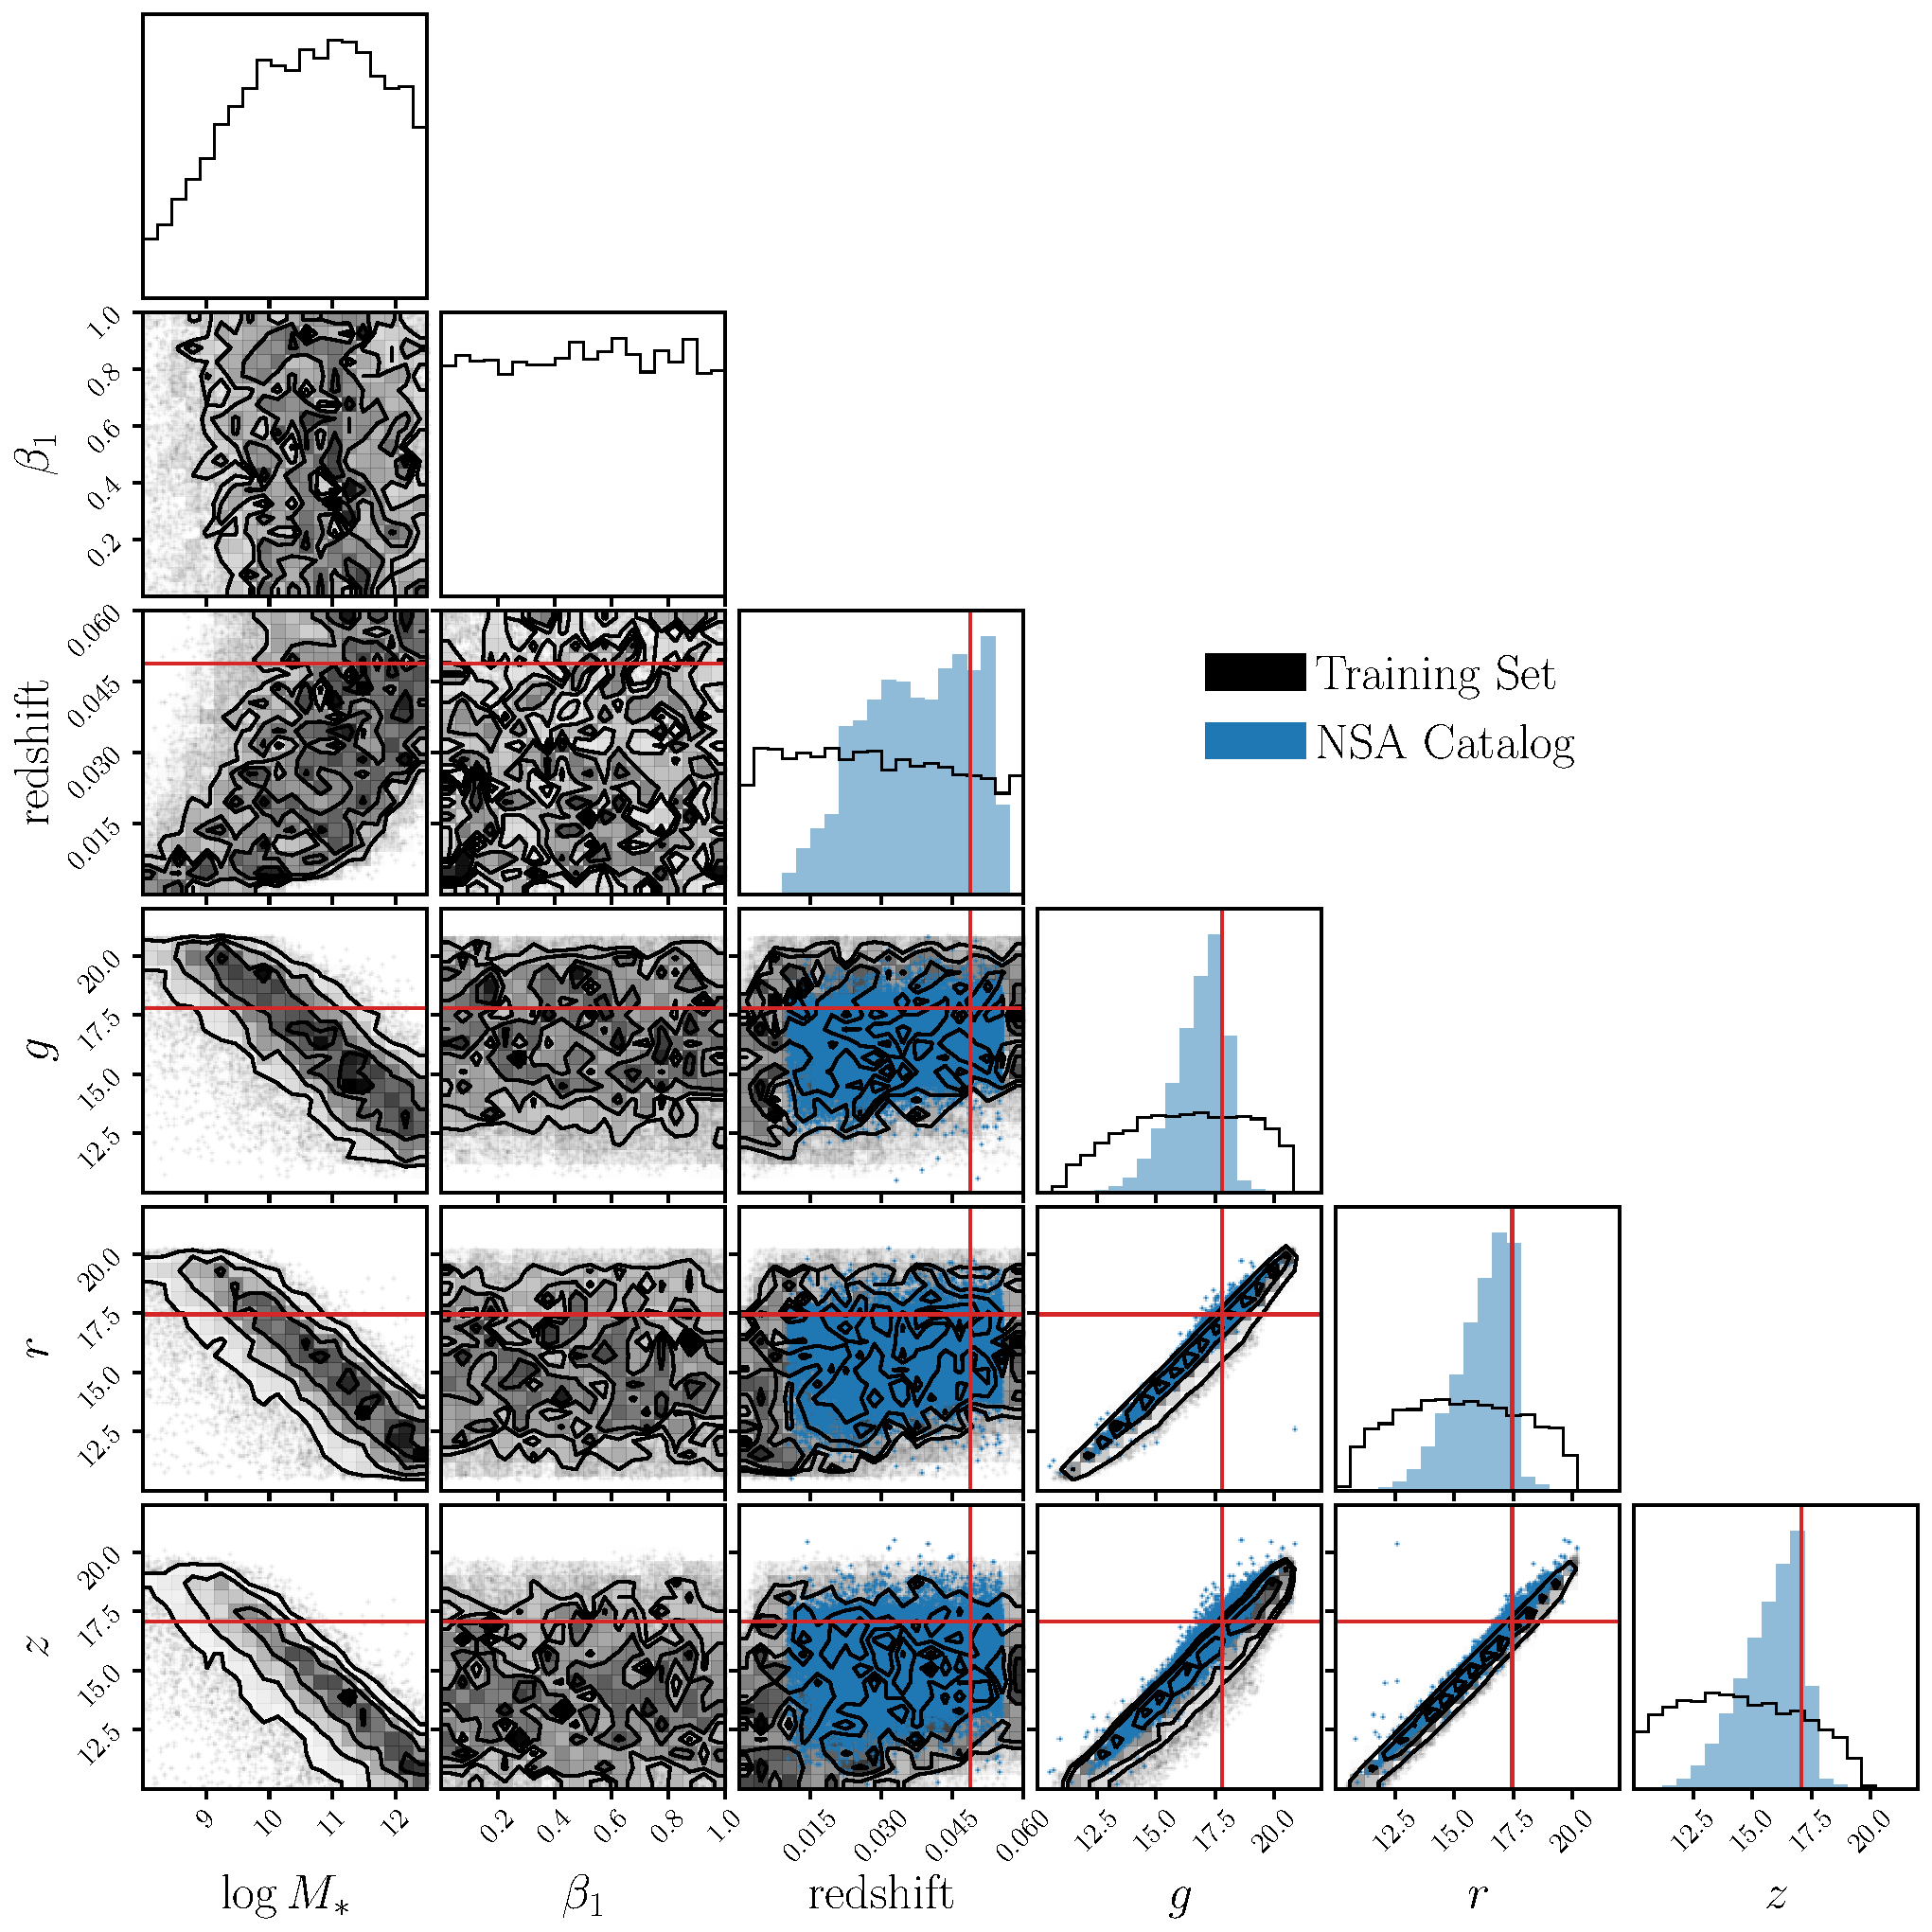
\includegraphics[width=0.9\textwidth]{figs/training.pdf}
    \caption{\label{fig:data}
    Joint distribution of SED model parameters, redshift, photometric
    magnitudes, and uncertainties of the data used to train \sedflow.
    We plot only a subset of the parameters ($\log M_*$, $\beta_1$) and
    photometric bands for clarity.
    The training data was constructed by sampling SED model parameter values
    from the prior and forward modeling optical photometry using the PROVABGS
    and noise models (Section~\ref{sec:sedflow}). 
    For comparison, we present the distribution of redshift, magnitudes, and
    uncertainties for galaxies in the NSA catalog (blue). 
    \emph{The training set fully encompasses the observations; thus, 
    {\sc SEDflow} can be used to infer the posterior for all NSA galaxies}.
    }
\end{center}
\end{figure}
%%%%%%%%%%%%%%%%%%%%%%%%%%%%%%%%%%%%%%%%%%%%%%%%%%%%%%%%%%%%%%%%%%%%%%%%%%%%
% training data 
%%%%%%%%%%%%%%%%%%%%%%%%%%%%%%%%%%%%%%%%%%%%%%%%%%%%%%%%%%%%%%%%%%%%%%%%%%%%
\subsection{Training Data} \label{sec:training}
In this section, we describe how to we construct the training data for
\sedflow~using the PROVABGS SED model.
First, we sample $N_{\rm train}$ SED model parameters from a prior: $\theta'\sim p(\theta)$. 
We use the same priors as \chedit{Hahn \etal~(2022)}: uniform priors over $M_*,
t_{\rm burst}, f_{\rm burst}, \gamma_1, \gamma_2, \tau_{\rm BC}, \tau_{\rm ISM},
n_{\rm dust}$ with broad conservative ranges and Dirichlet prior over $\beta_1,
\beta_2, \beta_3, \beta_4$, chosen to normalize the NMF SFH.
For each $\theta'$, we also uniformly sample a redshift within the range of the
NSA: $z' \sim \mathcal{U}(0., 0.2)$. 
Next, we forward model mock observables --- NSA optical photometry
(Section~\ref{sec:obs}). 
We calculate the rest-frame galaxy SED from PROVABGS and redshift it: 
$F(\lambda;\theta', z)$. 
Afterwards, we convolve $F$ with optical broadband filters, $R_X$, to generate
noiseless photometric fluxes:
\begin{equation}
    f_X(\theta', z') = \int F(\lambda;\theta', z') \, R_X(\lambda) \, {\rm d}\lambda
\end{equation}
The next step of the forward model is to apply noise. 
We assign photometric uncertainties, $\sigma'_X$, by sampling an estimate of
the true $p(\sigma_X | f_X)$ of NSA galaxies. 
Then, we apply Gaussian noise
\begin{equation} \label{eq:noise} 
    \hat{f}_X(\theta', z', \sigma'_x) = f_X(\theta', z') + n_X  \quad {\rm where}~n_X \sim \mathcal{N}(0, \sigma'_X)
\end{equation}
to derive the forward modeled photometric flux.

For our estimate of $p(\sigma_X | f_X)$, we use an empirical estimate of
$p(\sigma_X | f_X)$ based on NSA photometry and measured uncertainties. 
For each band, we separately estimate  
\begin{equation}
    \hat{p}(\sigma_X | f_X) = \mathcal{N}( \mu_{\sigma_X}(f_X), \sigma_{\sigma_X}(f_X))
\end{equation}
as a Gaussian in magnitude-space. 
$\mu_{\sigma_X}$ and $\sigma_{\sigma_X}$ are the median and standard deviation
of $\sigma_X$ as a function of $f_X$ that we estimate by evaluating them in
$f_X$ bin and interpolating over the bins. 
Any $\theta'$ that is assigned a negative $\sigma'_X$ is removed from our
training data. 
We also remove any training data with $f_X(\theta'$ outside the range of NSA
photometry. 
Although this is a simplicistic noise model, we emphasize that our choice of
noise model does not strongly affect the accuracy of the posteriors from
\sedflow.
This is because we design \sedflow~to include $\sigma_X$ in the conditional
statement of the posterior. 
Hence, our primary concern is that $\sigma'_X$ spans the observed $\sigma_X$
values. 
We discuss this further in Section~\ref{sec:discuss}.

In total, we constuct $N_{\rm train} = 1,131,561$ sets of SED parameters,
redshift, photometric uncertainty, and mock NSA photometry: 
$\{(\theta', z, \sigma'_X, \hat{f}_X \}$.
There are 12 SED parameters and photometry and uncertainties in 5 NSA bands. 
In Figure~\ref{fig:data}, we present the training data through the joint
distribution of a subset of $\{(\theta', z, \sigma'_X, \hat{f}_X \}$ (black).
We include select SED model parameters ($\log M_*$, $\beta_1$), redshift,
photometry ($g$ and $r$ bands), and photometric uncertainty ($r$ band).
We also include the distribution of redshift, photometry, and uncertainty of
NSA galaxies (blue).
The photometry and uncertainties are in magnitude-space. 
The distribution of the training data fully spans the distribution of NSA
galaxies.
Hence, the training data provides support over the full $(f_X, \sigma_X, z)$
space of the NSA observations. 
%and the trained ANPE can accurately estimate posteriors for all NSA galaxies. 

\subsection{Training \sedflow} \label{sec:anpe_train}
For \sedflow, we use a MAF normalizing flow model (Section~\ref{sec:flow}) with 
15 MADE blocks, each with 2 hidden layers and 500 hidden units.
In total, the model has 7,890,330 free hyperparameters, ${\bf h}$. 
We detremine this architecture through random hyperparameter search. 
Our goal is to determine ${\bf h}$ of the MAF model, 
$q(\theta\given\bfi{x}, {\bf h})$, so that it accurately estimates the
posterior probability distribution $p(\theta\given\bfi{x})$. 
$\theta$ represent the SED parameters and ${\bf x} = (f_X, \sigma_X, z)$.
We do this by minimizing the KL divergence between 
$q(\theta\given{\bf x}, {\bf h})$ and $p(\theta\given{\bf x})$:
$D_{\rm KL} (p\,||\,q)$. 

In practice, we split the training data (Section~\ref{sec:training}) into a
training and validation set with a 90/10 split. 
Afterwards, we maximize the total log likelihood $\sum_i \log q(\theta_i\given
\bfi{x}_i, \bf{h})$ over training set, which is equivalent to minimizing 
$D_{\rm KL} (p\,||\,q)$.
We use the {\sc Adam} optimizer~\citep{kingma2017} with a learning rate of $5\times10^{-4}$. 
To prevent overfitting, we evaluate the total log likelihood on the validation
data at every training epoch and stop the training when the validation log
likelihood fails to increase after 20 epochs.  
Training our model with a batch size of 50 takes roughly a day on a single 2.6
GHz Intel Skylake CPU. 
Given our small batch size, we find similar training times when using CPUs or
GPUs. 

\begin{figure}
\begin{center}
    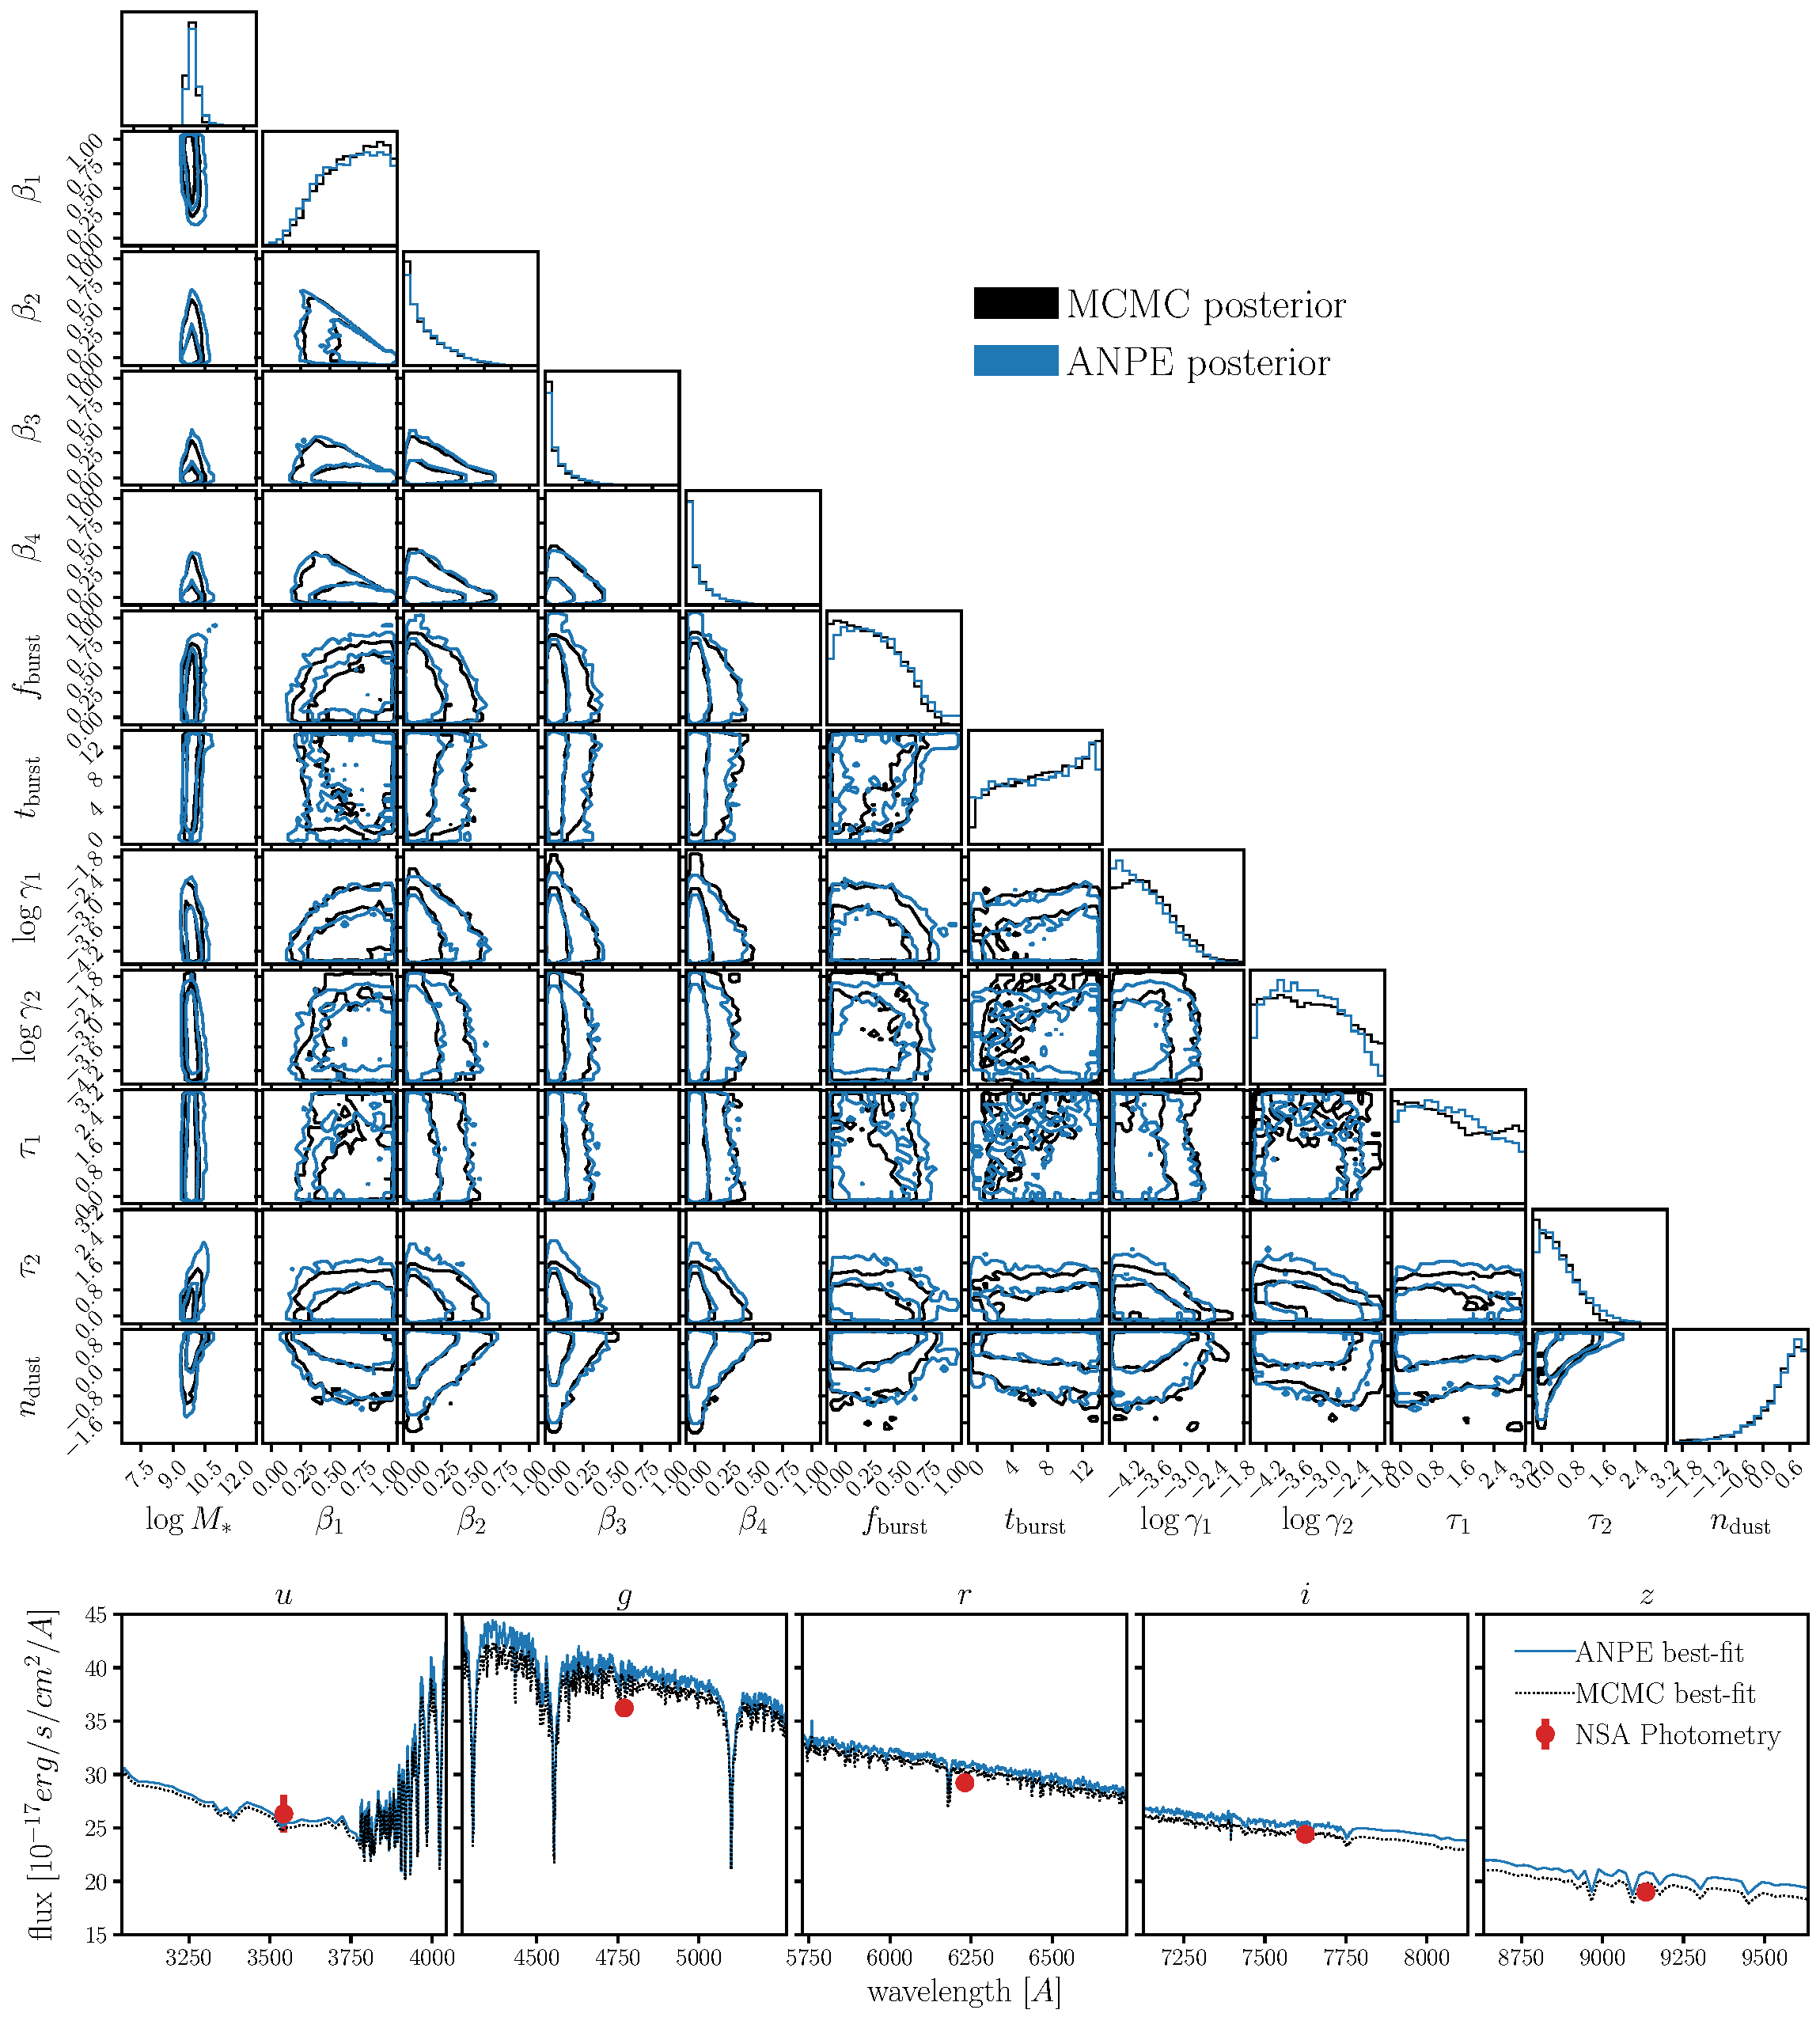
\includegraphics[width=0.9\textwidth]{figs/corner.pdf}
    \caption{\label{fig:corner}
    A comparison of the posteriors of the 12 SED model parameters derived from
    standard MCMC sampling (black) and our \sedflow~(blue) for an arbitrarily
    selected NSA galaxy ($\mathtt{NSAID} = 72$).
    The posteriors are in excellent agreement for all of the SED parameters. 
    In the bottom panel, we present the SEDs of the the best-fit parameter
    values from the \sedflow~(blue) and MCMC posteriors (black dotted), which
    are all in excellent agreement with the observed NSA photometric flux
    (red). 
    %We mark the optical broadband response curves (dashed) for reference. 
    Estimating the posterior using MCMC sampling requires 10 CPU hours. 
    Even using neural emulators to accelerate likelihood evaluations, MCMC
    sampling requires 10 CPU minutes. 
    \emph{With \sedflow, inferring the full posterior takes 1 second per
    galaxy.}
    }
\end{center}
\end{figure}

\section{Results} \label{sec:results}
Now that we have trained \sedflow, we can estimate the posterior,
$p(\btheta\given \bfi{x}_i)$, for any 
$\bfi{x}_i = \{f_{X,i}, \sigma_{X,i}, z_i \}$. 
In practice, we do this by drawing samples from the \sedflow~NDE model. 
Since we use a normalizing flow, this is trivial:
we generate samples from the target distribution of the normalizing flow,  a
multivariate Gaussian distribution in our case, then we transform the samples
using the bijective transformation in Eq.~\ref{eq:normflow} that we trained.
The transformed samples follow $p_\phi(\btheta\given \bfi{x}_i)$ and 
estimate the posterior, $p(\btheta\given \bfi{x}_i)$. 

Next, we validate the accuracy of the \sedflow~posterior estimates.
As a first test, we compare the posterior from \sedflow~to the posterior derived
from MCMC sampling for a single arbitrarily chosen NSA galaxy in
Figure~\ref{fig:corner} ($\mathtt{NSAID} = 72$). 
In the top, we present the the posterior distribution of the 12 SED model
parameters for the \sedflow~posterior (blue) and MCMC posterior (black). 
\emph{The \sedflow~posterior is in excellent agreement with the MCMC posterior
for all of the SED parameters}. 
 
In the bottom of Figure~\ref{fig:corner}, we compare the SEDs of the best-fit
parameter values from the \sedflow~(blue) and MCMC posteriors (black dotted). 
We also include the NSA photometric flux of the selected galaxy (red). 
The best-fit SED from the \sedflow~posterior is also in good agreement with
both the MCMC best-fit SED and the NSA photometry.  

% separate paragraph highlighting the computational advantage? 
The key advantage of ANPE is that it enables accurate Bayesian inference
orders of magnitude faster than conventional methods. 
We derive the MCMC posterior using the {\sc Zeus} ensemble
slice-sampler~\citep{karamanis2020} with 30 walkers and 10,000 iterations.
2,000 of the iterations are discarded for burn-in. 
In total, the MCMC posterior requires >100,000 SED model evaluations. 
Since each evaluation takes ${\sim}340$ ms, it takes ${\sim}10$ CPU hours for a
single MCMC posterior. 
Recently, SED modeling has adopted neural emulators to accelerate SED model
evaluations~\citep{alsing2020}. 
In \cite{hahn2022}, for instance, the PROVABGS emulator takes
only ${\sim}2.9$ ms to evaluate, >100$\times$ faster than the original model. 
Yet, even with emulators, due to the number of evaluations necessary for
convergence, an MCMC posterior takes ${\sim}10$ CPU minutes. 
Meanwhile, after training, \emph{the \sedflow~posterior takes $1$ second ---
>$10^4\times$ faster than MCMC}. 

\begin{figure}
\begin{center}
    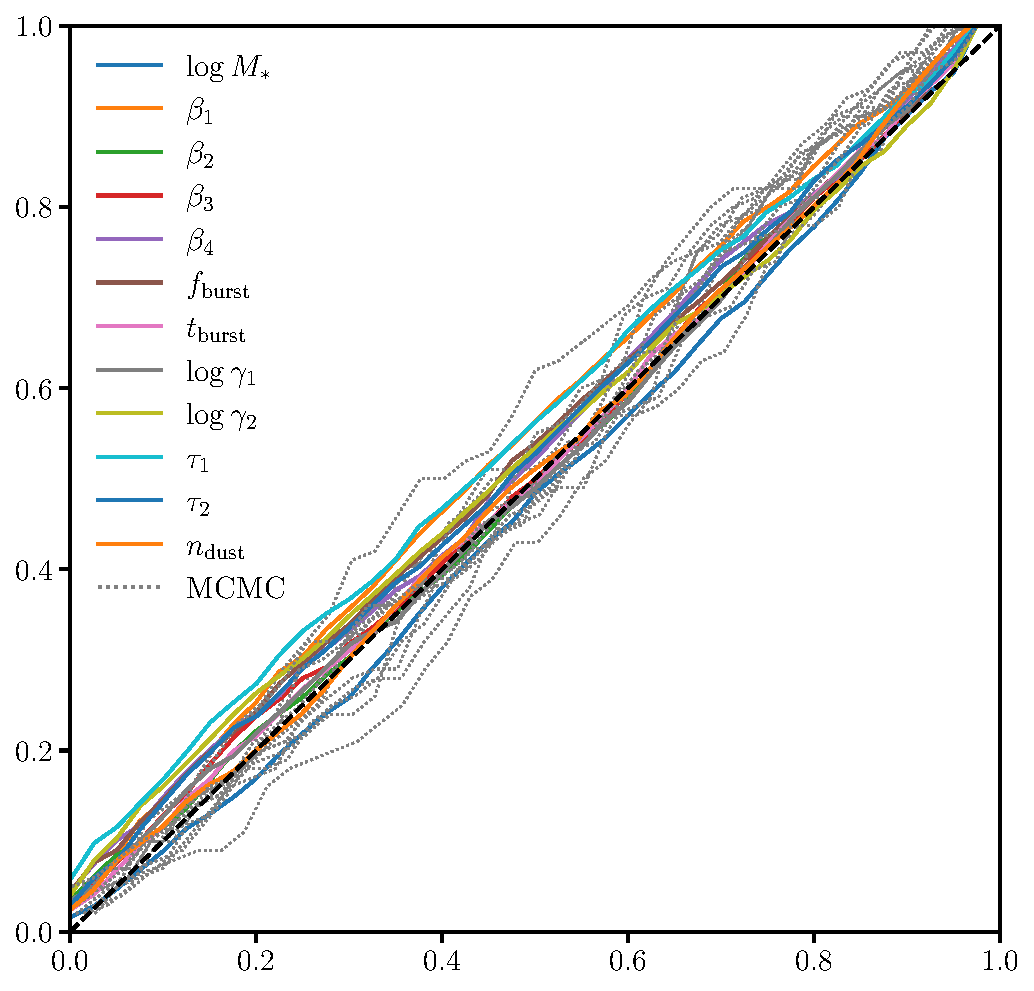
\includegraphics[width=0.5\textwidth]{figs/ppplot.pdf}
    \caption{\label{fig:pp}
    Probability-probability (p-p) plot of the \sedflow~posteriors for 1000
    synthetic test observations, with known true parameter values. 
    We plot the CDFs of the percentile score of the true values within the
    marginalized \sedflow~posteriors for each SED parameter.
    For the true posteriors, the percentile score is uniformly distributed so
    the CDF is diagonal (black dashed).
    %The test data is constructed in the same way as the training data (Section~\ref{sec:training}). 
    For reference, we include the p-p plot of the posterior estimated from MCMC
    sampling (gray). 
    \emph{The \sedflow~posteriors are in excellent agreement the true
    posteriors.}
    }
\end{center}
\end{figure}
The posteriors from \sedflow~and MCMC are overall in excellent for NSA
galaxies, besides the one in Figure~\ref{fig:corner}.
However, we do not know the true SED parameters for these galaxies so to
further validate \sedflow, we use test synthetic photometry, where we know the
truth.
We sample 1000 SED parameters from the prior,
$\{\btheta^{\rm test}_i\} \sim p(\btheta)$, 
and forward model synthetic NSA observations, 
$\{\bfi{x}^{\rm test}_i\}$, 
for them in the same way as the training data (Section~\ref{sec:training}). 
Afterwards, we generate posteriors for each of $\bfi{x}^{\rm test}_i$ using 
\sedflow: $\{ p(\btheta \given \bfi{x}^{\rm test}_i)\}$. 

In Figure~\ref{fig:pp}, we present the probability-probability (p-p) plot of
the \sedflow~posteriors for the test data. 
The p-p plot presents the cumulative distribution function (CDF) of the
percentile score of the true value within the marginalized posterior for each
parameter. 
For true posteriors, the percentiles are uniformly distributed so the CDF is a
diagonal (black dashed).
Overall, the CDFs for \sedflow~lie close to the diagonal for each of the SED
parameters. 
\emph{Hence, the \sedflow~posteriors are in excellent agreement with the true
posteriors}.

In Figure~\ref{fig:pp}, we also include the CDFs of the SED parameters for the
MCMC posteriors derived for a subset of 100 test observations (gray dotted). 
Comparing the CDFs from the MCMC posteriors to those of \sedflow, we find that
the \sedflow~posteriors are actually in better agreement with the true
posteriors. 
This is due to the fact that MCMC posteriors are also only estimates of the
true posterior and are subject to limitations in initialization, sampling, and
convergence.
Posteriors from \sedflow~are not impacted by these limations, so the comparison
highlights additional advantages of an ANPE approach besides the
${>}10^4\times$ performance improvement.

\begin{figure}
\begin{center}
    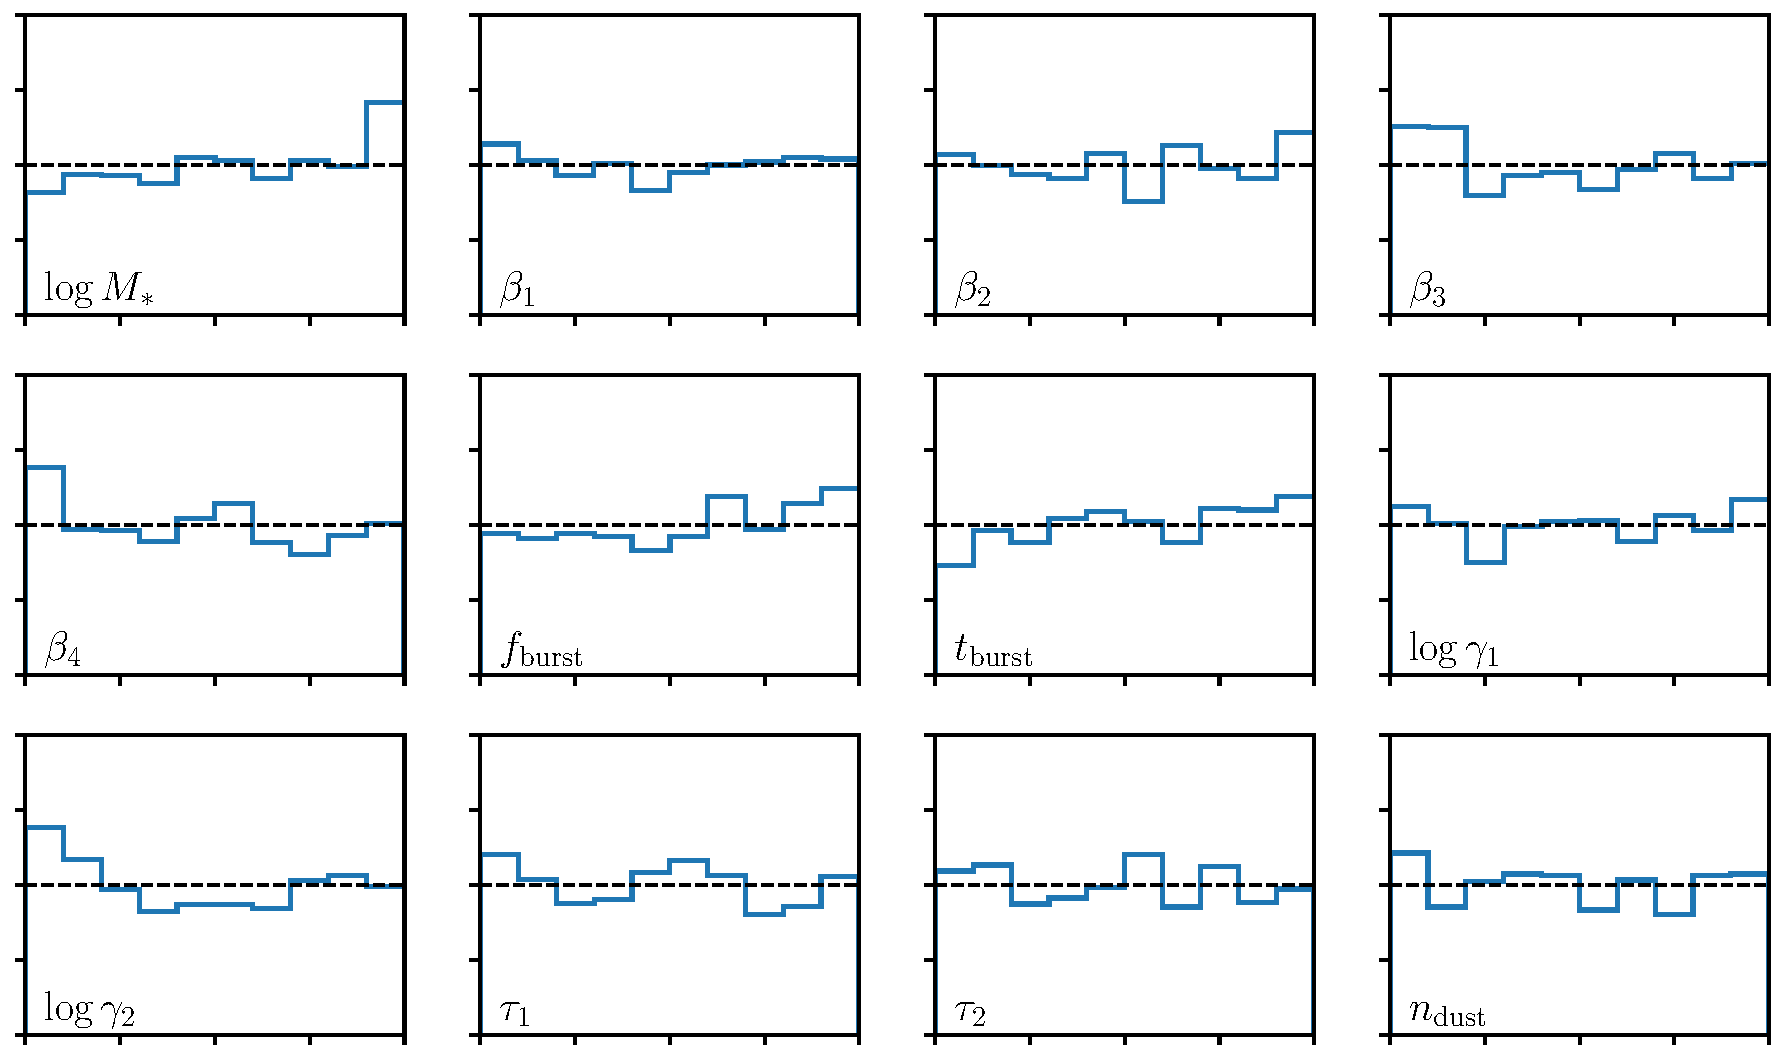
\includegraphics[width=0.9\textwidth]{figs/sbc.pdf}
    \caption{\label{fig:sbc}
    Simulation-based calibration plot of the \sedflow~posteriors for 1000
    synthetic test observations. 
    The histogram in each panel represents the distribution of the rank
    statistic of the true value within the marginalized \sedflow~posterior
    (blue) for each SED parameter.
    For the true posterior, the rank statistics will have a uniform
    distribution (black dashed). 
    For reference, we include the rank distribution of the MCMC posteriors for
    a subset of 100 test data (gray dotted). 
    The rank statistic distribution of \sedflow~is nearly uniform for all of
    the SED parameters. 
    Therefore, \emph{\sedflow~provides unbiased and accurate estimates of the
    true posteriors.}
    }
\end{center}
\end{figure}

We examine another validation of the \sedflow~posteriors using simulation-based
calibration~\citep[SBC;][]{talts2020}. 
Rather than using percentile scores, SBC examines the distribution of the rank
statistics of the true parameter values within the marginalized posteriors. 
It addresses the limitation that the CDFs only asymptotically approach the true
values and that the discrete sampling of the posterior can cause artifacts in
the CDFs. 
In Figure~\ref{fig:sbc}, we present SBC of each SED parameter for the
\sedflow~posteriors (blue) using the 1000 test observations.
For comparison, we include the SBC for the MCMC posteriors (gray dotted). 
Similar to the percentile score, the distribution of the rank statistic is
uniform for the true posterior (black dashed). 
The rank statistic distribution for the \sedflow~posteriors are nearly uniform
for all SED parameters. 
Hence, \emph{we confirm that the \sedflow~posteriors are in excellent agreement
with the true posterior}.

An advantage of SBC is that by examining the deviation of rank statistics
distribution from uniformity, we can determine how the posterior estimates
deviate from the true posteriors. 
For instance, if the distribution has a U-shape where the true parameter values
are more often at the lowest and highest ranks, then the posterior estimates
are narrower than the true posteriors.
If the distribution has a $\cap$-shape, then the posterior estimates are
broader than the true posteriors. 
Any asymmetry in the distribution implies that the posterior estimates are
biased.  
For the \sedflow~posteriors, we find none of these features for any of the SED
parameters. 
Hence, \sedflow~provides unbiased and accurate estimates of the true posteriors
for all SED parameters. 

With the accuracy \sedflow~validated, we apply it to derive posteriors for all
of our NSA galaxies (Section~\ref{sec:obs}). 
Analyzing all 33,883 NSA galaxies takes <12 CPU hours. 
For each galaxy, we generate 10,000 samples of the 12-dimensional posterior,
$p(\btheta \given \bfi{x})$. 
These posteriors on SED parameters represent posteriors on stellar mass, SFH,
ZH, and dust content of the NSA galaxies. 
To maximize the utility of the posteriors further, we use them to derive
posteriors on the following additional galaxy properties: SFR averaged over
1Gyr, mass-weighted metallicity, and mass-weighted stellar age (see
Eq. 17 in \citealt{hahn2022} for the exact calculation).
We publicly release all of the posteriors for our NSA sample at 
\url{some-url-here}. 
Furthermore, \sedflow~model and all of the software used to train it are
publicly available at \url{https://github.com/changhoonhahn/SEDflow/}. 

\section{Discussion} \label{sec:discuss}
\subsection{Further Validation} 
In the previous section, we validated and demonstrated the accuracy of
\sedflow~posteriors. 
Nevertheless, a primary determining factor of \sedflow, and any ML model, is
the quality of the training data.
In our case, the training data is generated using a forward model with two
components: the PROVABGS SED model and a noise model
(Section~\ref{sec:training}).
We first consider the noise model. 

In our noise model, we assign noiseless photometric fluxes uncertainties based
on an empirical estimate of $p(\sigma_X\given f_X)$ for each band
independently. 
Afterwards, the assigned $\sigma_X$ is used to apply Gaussian noise to the
photometric flux (Eq.~\ref{eq:noise}). 
This is a simplicistic noise model and, as the bottom right ($g - \sigma_r$ and
$r - \sigma_r$) panels of Figure~\ref{fig:data} reveal, there are discrepancies
in the magnitude versus uncertainty distributions of the training data and
observations. 
Despite these discrepancies, \sedflow~provides excellent estimates of the true
posterior.  
This is because we design our ANPE to include $\sigma_X$ as a conditional
variable (Section~\ref{sec:anpe_train}).
The $f_X-\sigma_X$ distribution of our training data does not impact the
accuracy of the posteriors as long as there is sufficient training data near
$\xobs$ to properly train the NDE in the region.

A more accurate noise model will, in theory, improve the performance of
\sedflow~since the $\bfi{x}$-space of the training data will more effectively
span the observations. 
In other words, there will be fewer training data expended in regions of 
${\bf x}$-space that are devoid of observations.  
However, for our application to SED modeling, we do not find significantly  
improved performance when we replace the noise model.
This suggests that even with our simplicistic forward model, the
$\bfi{x}$-space of observations is sufficiently covered by the training data. 
We note that when we decrease $N_{\rm train}$ below 500,000,
\sedflow~posteriors are significantly less accurate. 
A more realistic forward model may reduce this $N_{\rm train}$ threshold for
accurate posteriors. 
However, generating $N_{\rm train} \sim 1,000,000$ training has a negligible
computational cost compared to MCMC SED modeling so we do not explore this
further. 

Next, we consider limitations in the PROVABGS SED model used in our forward
model. 
One of its advantages is that it uses a compact and flexible prescription for
SFH and ZH that can describe a broad range of SFHs and ZHs.
However, the prescription was derived from simulated Illustris galaxies, whose
SFHs and ZHs may be not reflect the full range of SFHs and ZHs of real galaxies.
If certain subpopulations of galaxies have SFHs and ZHs that cannot be
described by the PROVABGS prescriptions, they cannot be accurately forward
modeled. 
Furthermore, even if the PROVABGS SFH and ZH prescriptions are sufficient,
there are limitations in our understanding of stellar evolution. 

There is currently no consensus in the stellar evolution, stellar spectral
libraries, or IMF of galaxies~\citep[\emph{e.g.}][]{treu2010, vandokkum2010,
rosani2018, ge2019, sonnenfeld2019}.
The PROVABGS model uses MIST isochrones, \cite{chabrier2003} IMF, and the MILES
+ BaSeL spectral libraries. 
These choices limit the range of SED that can be produced by the training data. 
For instance, if galaxies have significant variations in their IMF, assuming a
fixed IMF would reduce the range of our training data.  
A more flexible SED model that includes uncertainties in SPS would broaden the
range of galaxy SEDs that can be modeled.
Data-driven approaches may also enable SED models to be more
descriptive~\citep[\emph{e.g.}][]{hogg2016, portillo2020}. 
Improving  SED models, however, is beyond the scope of this work. 
Our focus is on improving the Bayesian inference framework.
In that regard, the limitations of the SED model equally impacts conventional
approaches with MCMC. 

%\todo{revisit paragraph below after applying sedflow to NSA} 
%Although we demonstrate that \sedflow~produces accurate posteriors for $\xobs$
%within the $\bfi{x}$ support of the training data, there are a few objects in
%the NSA catalog are outside of the support. 
%For instance, the $g$, $r$, $\sigma_r$ panels of Figure~\ref{fig:data} reveal a
%number of NSA objects (blue) that lie outside of the $g-r$ color distribution
%of the training data (black). 
%This is not due to deficiencies in the noise model since the $g-\sigma_r$ and
%$r-\sigma_r$ relations of these NSA objects are within that of the training 
%data. 
%Some of these objects are likely observational artifacts. 
%Even with the quality cuts in Section~\ref{sec:obs}, there are likely objects
%in our samples with problematic photometry.  
%\chedit{list a few typical examples of problematic photometry}. 
%The SEDs of such artifcats cannot be modeled using an SPS model combined with
%noise, so they can lie outside of the training ${\bf x}$ support.

%In Section~\ref{sec:results}, we assessed the accuracy of the \sedflow~posteriors using posteriors derived using MCMC and test observations, where we know the true parameter values. 
%Both cases demonstrate the high level of accuracy of \sedflow.  However, for applications that require even higher fidelity posteriors, there are further tests. 
Given the limitations of any forward model, we can construct additional tests
of posteriors derived from ANPE. 
For instance, the $\chi^2$ of the best-fit parameter value from the 
estimated posterior can be used to test whether the best-fit model 
accurately reproduces observations.
This would only require one additional model evaluation. 
As another test of the posteriors, one can construct an Amortized Neural
Likelihood Estimator (ANLE) using the same training data. 
Unlike the ANPE, which estimates $p(\theta\given f_X, \sigma_X, z)$, the ANLE
would estimate $p(f_X \given \theta, \sigma_X, z)$.
We can then further validate the posteriors by assessing whether the observed
photometry lies within the ANLE. 
Based on the high level of accuracy of \sedflow~posteriors in the previous
section, we do not explore these additional tests; however, they can be used to
further validate any ANPE posterior. 

\subsection{Additional Advantages} 
So far, we have primarily focused on the computational advantages of
\sedflow~for individual posterior estimation. 
However, there are other benefits to our ANPE approach. 
One of the key ingredients in Bayesian inference is the prior. 
For SED modeling, recent works have demonstrated that model priors play a
crucial role in the derived galaxy properties~\citep{carnall2018, leja2019,
hahn2022}. 
Even ``uniformative'' uniform priors on SED model parameters can impose
undesirable priors on derived galaxy properties such as $M_*$, SFR, SFH, or
ZH.
This underscores the importance of carefully selecting priors and validating
results using multiple different priors. 
For SED modeling with MCMC, selecting a different prior requries reevaluating
every posterior and repeating all the SED model evaluations in the MCMC
sampling.  
For ANPE, the prior is set by the distribution of parameters in the training
data. 
For a new prior, instead of regenerating the training data, we can subsample
it so that the parameters follow the new prior. 
Afterwards, the ANPE model can be re-trained, re-validated on the test data,
and re-deployed on observations.
Each of these steps require substantially less computational resources than
generating a new set of training data or using MCMC methods. 
Hence, the ANPE approach also provides a way to efficiently vary the prior
without multiplying computational costs. 

In this work, we use \sedflow~to perform SED modeling on galaxy photometry. 
We estimate a 12-dimensional probability distribution with an 11-dimensional
conditional variable space. 
While this dimensionality is already a limiting factor for current MCMC
methods, ANPE has already been applied to higher dimensional applications.
\cite{dax2021}, for instance, constructed an accurate ANPE for a
15-dimensional model parameter space and 128-dimensional conditional variable
space.
Furthermore, NDE is an actively developing field in ML and new and methods are
constantly emerging~\citep[\eg][]{wu2020, dhariwal2021}. 

Without the limitations of current Bayesian inference methods, ANPE opens the
doors to better SED modeling. 
As mention above, SED models currently do not account for uncertainties in
stellar evolution, spectral libraries, or the IMF. 
Since ANPE approaches can handle higher dimensionality, SED models can include 
additional parameters that model these uncertainties as well as any
observational systematics (\emph{e.g.} zero-point calibration). 

\subsection{Subsequent Applications} 
In this work, we apply the ANPE approach to optical photometry, photometric
uncertainties, and redshifts from the NSA. 
Our approach can easily be extended beyond this application. 
For instance, we can include multi-wavelength photometry at ultra-violet (UV)
or infrared (IR) wavelengths. 
We can also modify \sedflow~to infer redshift from photometry. 
In \sedflow, we include redshift as a conditional variable, since NSA provides
spectroscopic redshifts. 
However, redshift can be included as an inferred variable rather than a
conditional one. 
Then, we can apply \sedflow~to infer galaxy properties from photometric data
sets without redshift measurements while marginalizing over the redshift
prior. 
If we do not require spectroscopic redshifts, \sedflow~can be extended to much
larger data sets that span fainter and broader galaxy samples. 
Conversely, we can use \sedflow~to infer more physically motivated photometric 
redshifts, where we marginalize over our understanding of galaxies rather than
using templates. 

The ANPE approach to SED modeling can also be extended to galaxy spectra. 
Constructing an ANPE for the full data space of spectra, however, requires
estimating a dramatically higher dimensional probability distribution. 
SDSS spectra, for instance, have ${\sim}3,600$ spectral elements.  
Furthermore, in our approach we include the uncertainties of observables as
conditional variables, which double the curse of dimensionality.
Recent works, however, have demonstrated that galaxy spectra can be represented
in a compact low-dimensional space using autoencoders~\citep[][; Melchior \&
Hahn in prep.]{portillo2020}.
In \cite{portillo2020}, they demonstrate that SDSS galaxy spectra can be
compressed into 10-dimensional latent variable space with little loss of
information. 
Such spectral compression dramatically reduces the dimensionality of the
conditional variable space to dimensions that can be tackled by current ANPE
methods. 
We will explore SED modeling of galaxy spectrophotometry using ANPE and
spectral compression in a following work. 

With \sedflow, we can generate accurate posteriors for SED modeling >$10^4$
faster than conventional MCMC methods. 
Analyzing 33,887 NSA galaxies only takes \chedit{X} CPU hours.
Analyzing the 10 million galaxies of DESI BGS would only take ${\sim}3000$ CPU
hours.
An ANPE approach will enable rigorous SED modeling on the enormous galaxy
samples that will be observed by DESI, PFS, Rubin, JWST, and Roman. 
The Rubin observatory, alone, will soon provide photometry from billions of
galaxies. 
We will be able to construct probabilistic catalogs that provide accurate
posteriors on the physical properties for all of these galaxies. 

In addition to accurately measuring galaxy properties, these probabilistic
catalogs will enable new class of statistical techniques.
For instance, they can be used for population inference to derive the
distribution of galaxy properties for galaxy populations by combining
individual posteriors~\citep[\eg][]{leja2019a}.
With probabilistic catalogs, we can also robustly probe less explored, low
signal-to-noise, regimes that may shed new light on galaxy evolution, 
\eg~dwarf galaxies.
Since posteriors accurately quantify uncertainty, analyses can include galaxies
with less tightly constrained properties without introducing bias. 
We can also more reliably quantify the extreme or outlier galaxies.
These catalogs can also take advantage of Bayesian Hierarchical approaches that
improve the statistical power of observations through Bayesian shrinkage. 
Overall, these probabilistic catalogs will enable a new level of statistical
robustness in galaxy studies and more fully extract the statistical power of
future observations. 

\section{Summary} \label{sec:summary}
By analyzing the SED of a galaxy, we can infer detailed physical properties
such as its stellar mass, star formation rate, metallicity, and dust content. 
These properties serve as the building blocks of our understanding of how
galaxies form and evolve. 
Current state-of-the-art SED modeling methods use MCMC sampling to perform 
Bayesian statistical inference. 
They derive posterior probability distributions of galaxy properties given
observation that accurately estimate uncertainties and parameter degeneracies. 
Posteriors also enable marginalization over any nuisance parameters. 
For the dimensionality of current SED models, this requires ${\gtrsim}100,000$
model evaluations and take ${\gtrsim}10-100$ CPU hours per galaxy. 

Upcoming galaxy surveys, however, will observe \emph{millions} of galaxies
using \emph{e.g.} DESI, PFS, Rubin observatory, James Webb Space Telescope, and
the Roman Space Telescope. 
Analyzing all of these galaxies with current Bayesian SED models is infeasible
and would require \emph{billions} of CPU hours. 
Furthermore, computational costs will only multiply as SED models increase in 
sophistication and treat theoretical uncertainties more flexibly. 
Therefore, rigorous inference will soon be a major bottleneck for galaxy
studies. 

In this work, we present 
\begin{itemize}
\item we present galaxy SED modeling using ANPE and the recent provabgs sed model 
some detail about training 
Using a trained ANPE, we derive posteriors of galaxy properties in  1 second
\item We demonstrate the
We apply our ANPE SED modeling on test mock observations and compare them to
posteriors derived using MCMC sampling. 
\item we apply ANPE to infer posteriors of galaxy properties. 
For each galaxy, we infer posteriors of $M_*$, SFR, mass-weighted stellar
metallicity, mass-weighted age. 
The catalog of posteriors is publicly available at \url{urlhere}
\end{itemize}

In this work, we focus on SED modeling of optical photometry. 
Next step is to explore galaxy spectra. 
some more discussions 


\section*{Acknowledgements}
It's a pleasure to thank 
    Adam Carnall, 
    Miles Cranmer, 
    Kartheik Iyer,
    Andy Goulding,
    Jenny E. Green,
    Uro{\u s}~Seljak,
    Michael A. Strauss, 
    ...
for valuable discussions and comments.

\appendix
%\bibliographystyle{mnras}
\bibliography{sedflow} 
\end{document}
